\section{Data Preparation}\label{sec:data_preparation}

After the previous analysis, we proceeded to the data preparation stage, where the dataset was refined for the modelling phase.

\subsection{Question 1}

We began by importing the complete raw dataset and applied the results of our previous analysis to select the most relevant features.

First, we removed unnecessary variables according to the following criteria:
\begin{itemize}
    \itemsep0em
    \item Variables with more than 70\% missing values.
    \item Students from England, due to differences in their education system.
\end{itemize}

\noindent
Next, we introduced the following variables:
\begin{itemize}
    \itemsep0em
    \item \texttt{Avg Math Result}
    \item \texttt{Avg Reading Result}
    \item \texttt{Avg Science Result}
\end{itemize}

\noindent
These were calculated as the average of the respective plausible values (PV1 to PV10) for each student.
We also removed the subscales of Mathematics, as their information is already captured by the aggregated Math Result score.

Then, we grouped the \texttt{Country (CNT)} variable into three categories to reduce high dimensionality:
\begin{itemize}
    \itemsep0em
    \item Above Average
    \item Average
    \item Below Average
\end{itemize}
This grouping was based on the average performance of students in each country across all subjects.

Using this new cleaned dataset, we created a correlation chart to visualize which features have a strong correlation with the target variable \texttt{Avg Math Result}.
In Figure \ref{fig:correlation_chart_repeating} and Figure \ref{fig:correlation_chart_not_repeating}, we can see the correlation obtained for the non-repeating and repeating students, respectively.

\begin{figure}[H]
    \centering
    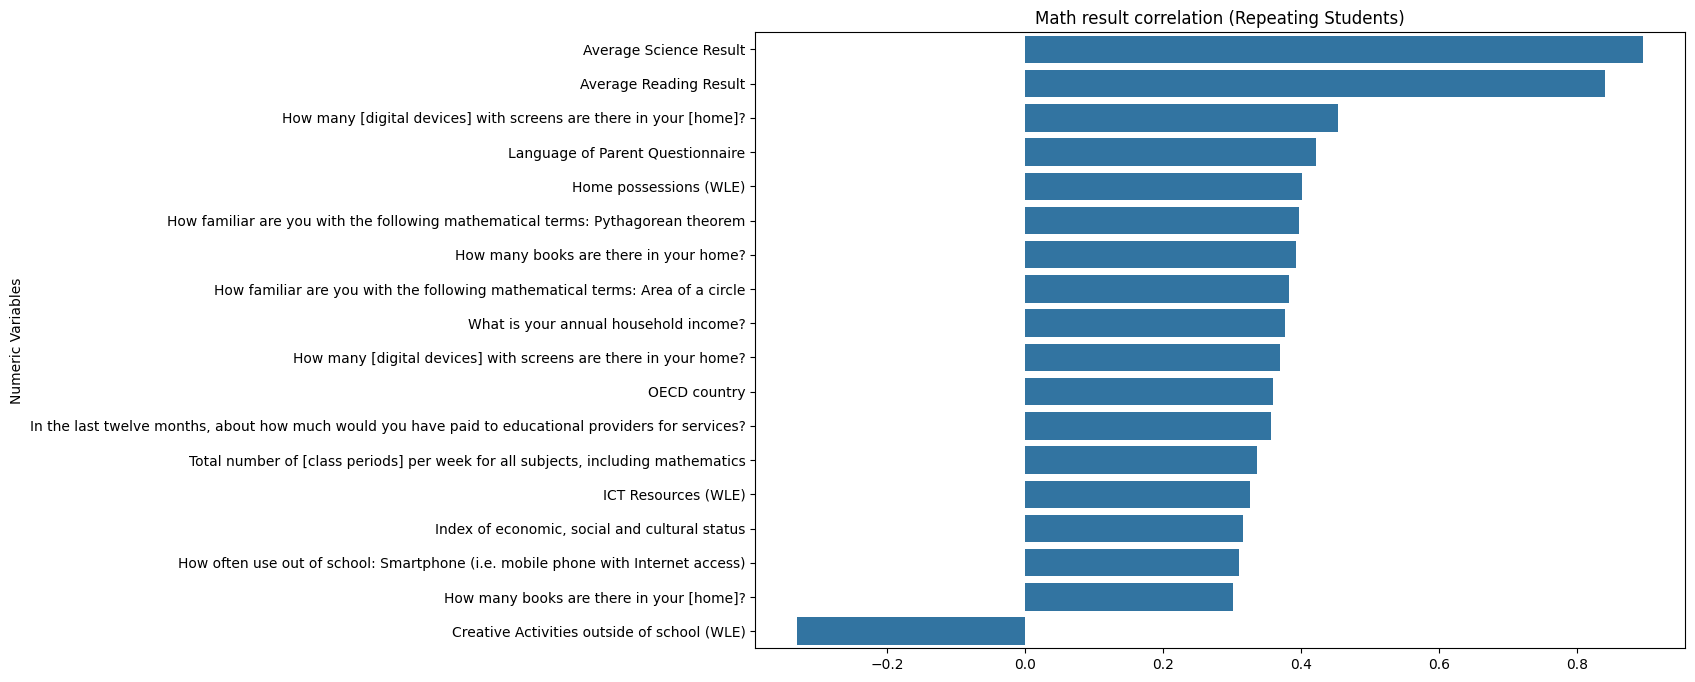
\includegraphics[width=0.48\textwidth]{figures/Q1_repratingcorrelations.png}
    \caption{Correlation matrix showing the relationship between selected features and the target variable \texttt{Avg Math Result} for repeating students.}
    \label{fig:correlation_chart_repeating}
\end{figure}


\begin{figure}[H]
    \centering
    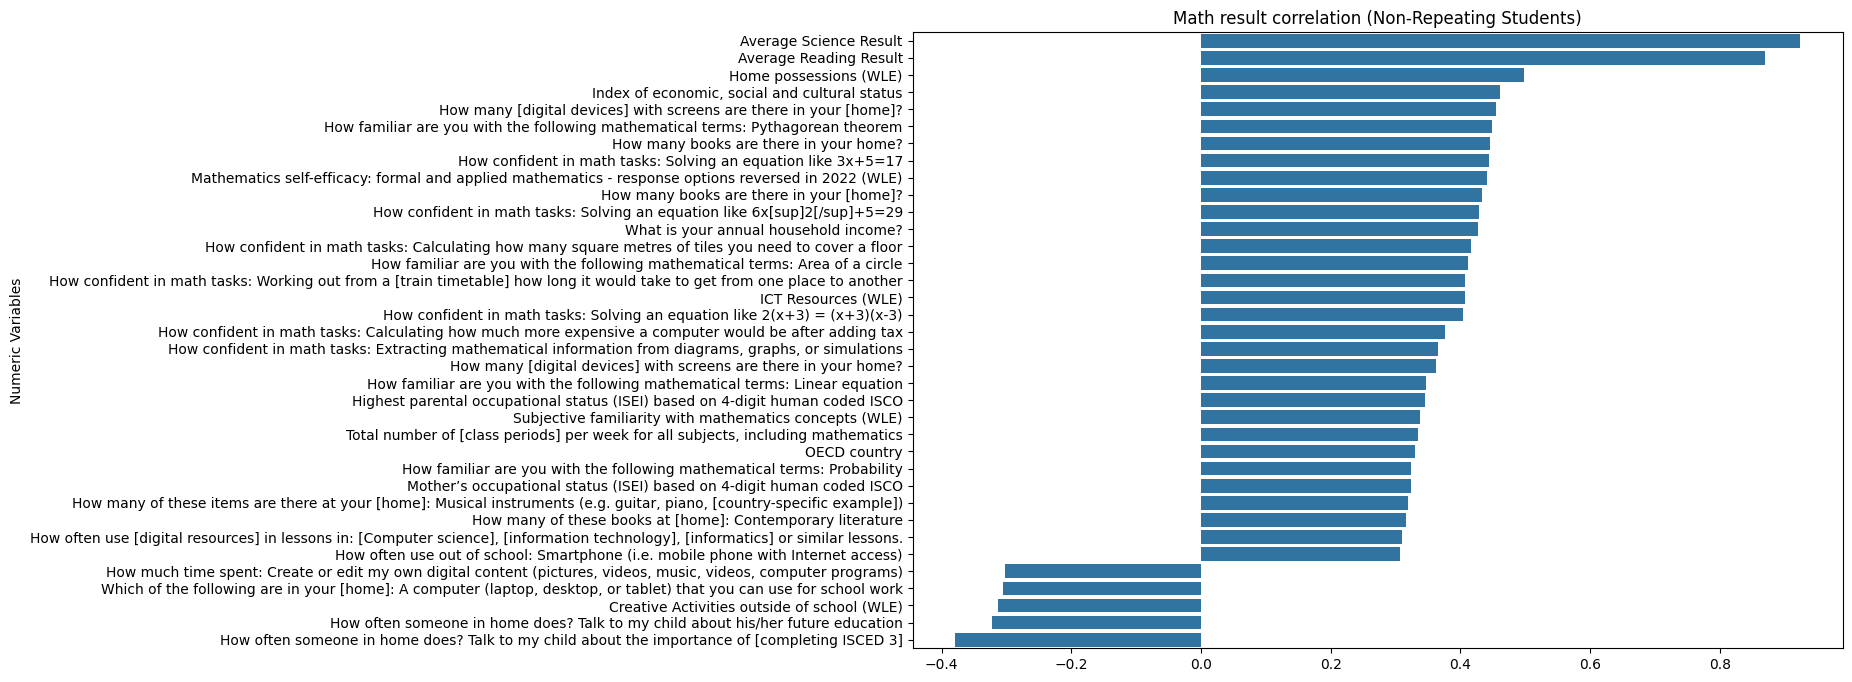
\includegraphics[width=0.48\textwidth]{figures/Q1_nonrepeatingcorrelations.png}
    \caption{Correlation matrix showing the relationship between selected features and the target variable \texttt{Avg Math Result} for non repeating students.}
    \label{fig:correlation_chart_not_repeating}
\end{figure}


Based on this analysis, we selected a mix of features that were significantly correlated with the target variable in either group. Additionally, we included the \texttt{Country (CNT)} variable to account for geographic effects.
The resulting dataset contains 34 variables and 600 772 rows of data, and serves as the foundation for the modelling phase.